
This chapter builds the foundation for the thesis introducing relevant concepts and disciplines for the thesis. 


Section \ref{evaluationofmatrix} provides an evaluation of the Matrix security model. The security model is evaluated in the context of a secure messaging system.  
The paper \emph{SoK: Secure Messaging} describes a evaluation framework for evaluating secure messaging systems. They define several security properties related to such systems \cite{sok} which will be presented.


All secure messaging systems with end-to-end encryption are based on the Double Ratchet algorithm from the Signal Protocol which will also be described.


Finally the architecture of Matrix and concepts related to Information-Flow Control will be introduced.

\section{Information security}

Information security is the discipline of protecting information. The key principles in information security are expressed through the CIA model. For a system to be secure these principles should be guaranteed \cite{michael2012}.

\begin{figure}[H]
	\centering
	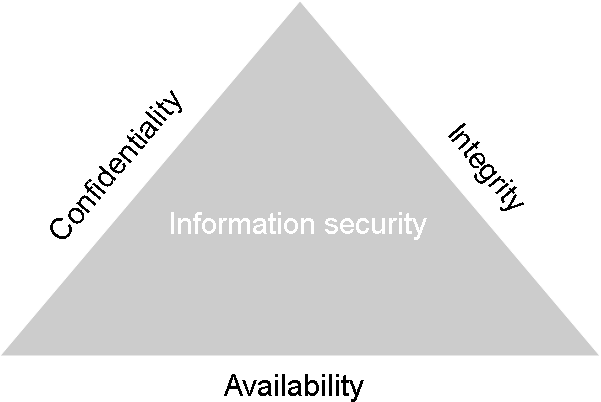
\includegraphics[width=10cm]{figures/cia.png}
	\caption{CIA triad}
	\label{fig:CIA triad}
\end{figure}


\subparagraph{Confidentiality}
Confidentiality is keeping information secret from unauthorized people. This is a major goal in information security. Encryption and access control are common ways of ensuring confidentiality \cite{michael2012}.

In a secure messaging system confidentiality would be guaranteed if the message being sent is only readable by the recipient and no one else \cite{sok}.

\subparagraph{Integrity}
Integrity is providing that information is unaltered and can only be changed by authorized people. If information is intercepted and changed during transit it would be a violation of integrity \cite{michael2012}.  
More specifically for a secure messaging it would mean that no altered message is accepted by the recipient \cite{sok}.

\subparagraph{Availability}
Making sure that information is accessible to authorized people is the goal of availability. Denial of Service attack \footnote{https://en.wikipedia.org/wiki/Denial-of-service\_attack} are common attacks targeting availability. 

Availability is generally more related to the system being available where the information itself plays a minor role \cite{michael2012}.
\\
\\
Depending on the type of system other properties must be satisfied as well. 


\subsection{Security properties}
The goal in a secure messaging system is to protect the messages being sent. The following properties are related to protecting messages.


\subparagraph{Authentication}
When a message is received the participant can verify that the message was sent from the actual sender. Furthermore a participant will receive evidence from a participant in a conversation that hey hold a known long-term secret. 



\subparagraph{Perfect Forward Secrecy}
If all keys are compromised than the decryption of any previously sent message should not be possible. Hence all previous messages would be secure however all future messages would be insecure 

\begin{figure}[H]
	\centering
	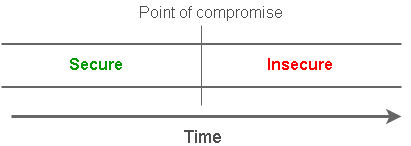
\includegraphics[width=10cm]{figures/forwardsecrecy.png}
	\caption{Forward secrecy}
	\label{fig:forward}
\end{figure}

\subparagraph{Backward secrecy}
If all keys are compromised than the decryption of \emph{future} messages should be possible. This property also goes by the names \emph{future secrecy} and \emph{post compromise security}. 

\begin{figure}[H]
	\centering
	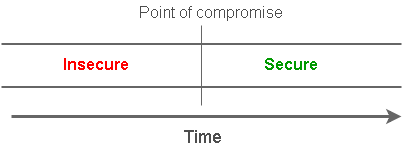
\includegraphics[width=10cm]{figures/backwardsecrecy.png}
	\caption{Backward secrecy}
	\label{fig:backward}
\end{figure}


\subsubsection{Other security properties}


\subparagraph{Participant Consistency} 
Whenever a message is accepted by a participant all participants are guaranteed to have identical view of the participant list.

\subparagraph{Destination Validation}
When a participant receives a message it can be verified that the participant was the intended recipient.

\subparagraph{Anonymity Preserving} 
The anonymity of the participants should be preserved and not linking any key identifiers.

\subparagraph{Speaker Consistency} 
There is consensus among the participants on the sequence of messages they receive by each participant. There might be a mechanism for checking consistency whenever a message is sent or after it has been received.

\subparagraph{Causality Preserving}
Messages must not be displayed before the message that originally precedes it has been displayed.

\subparagraph{Global Transcript} 
A global order where all messages are viewed in the same order for all participants.

\subparagraph{Deniability}
Deniability is a property where other participants cannot confirm that the message being sent was from the sender. Yet during the conversation there will be assurance for the recipient that the message being sent was authentic and sent by the sender \cite{sok}.

\begin{itemize}
	\item \emph{Message Unlinkability:} A deniability property that gives no guarantees that if a participant sent a message that other messages was sent by that participant as well. 
	\item \emph{Message Repudiation:} It can not be proved that a message was authored by a participant given the conversation transcript and all cryptographic key material. 
	\item \emph{Participant Repudiation:} It can not be proved that a participant was in a group conversation without his conversation transcript and cryptographic key material. 
\end{itemize}

The following properties are also defined in the paper \emph{SoK: Secure Messaging} but are less relevant for security.

\subparagraph{Group}

\begin{itemize}
	\item \emph{Computational Equality:} The computational load is equal for all participants.
	\item \emph{Trust Equality:} There is equal trust among all participants. 
	\item \emph{Subgroup messaging:} In the same conversation a participant can send messages to a subset of the participants.
	\item \emph{Contractible Membership:} When a participant leaves a conversation the protocol does not need to restart.
	\item \emph{Expandable Membership:} When a participant joins a conversation the protocol does not need to restart.
\end{itemize}

\subparagraph{Adoption}

\begin{itemize}
	\item \emph{Out-of-Order Resilient:} Messages received out-of-order should be accessible when received.
	\item \emph{Dropped Message Resilient:} On a unreliable network messages might be dropped in transit however it should not prevent decryption of future messages.
	\item \emph{Asynchronous:} Messages can be sent securely to recipients while they are offline.
	\item \emph{Multi-Device Support:} A participant can have multiple devices in a conversation and each device must be synchronized and should have the same historical conversation view
	\item \emph{No Additional Service:} There is no requirement of additional infrastructure being setup other than the participants. 
\end{itemize}





\newpage

\subsection{Concepts}

\subsubsection{Diffie-Hellman Key Exchange}

Diffie-Hellman is a key exchange protocol to establish a shared secret over an insecure channel. Public information is send over an insecure and using asymmetric keys two parties can derive the same shared key.


The first step is to agree on some public values. Either of the parties start the protocol by picking a large prime \emph{p} and a integer \emph{g} then the values are sent over the insecure channel.  

\begin{figure}[H]
	\hspace*{-1cm} 
	\centering
	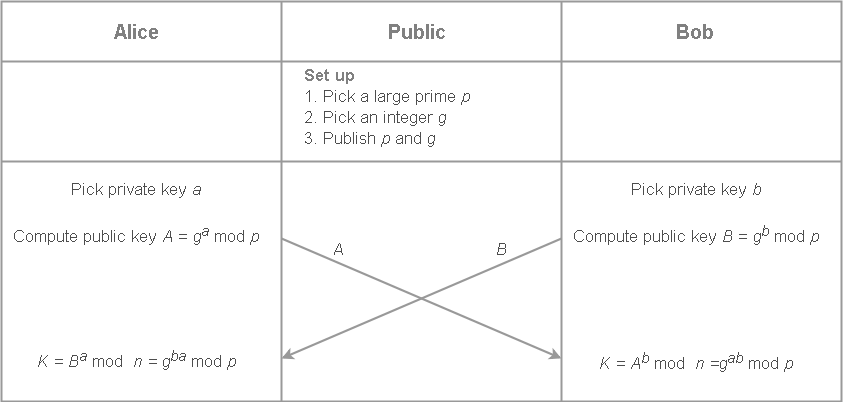
\includegraphics[width=14cm]{figures/dh.png}
	\caption{Simple Diffie-Hellman Key Exchange}
	\label{fig:dh}
\end{figure}

Alice and Bob will each pick a private key value and compute a public key value. The computed key value is sent over the insecure channel and Alice and Bob will both perform the same computation as previously \cite{crypto101}.


The Diffie-Hellman is vulnerable to man in the middle attack since there is no authentication taking place. There exist a solution to this problem using asymmetric key pairs and signing the messages being sent \cite{crypto101}.

\subsubsection{Key Derivation function}

Assume a secret key is established between two parties and is used to encrypt messages and exchange them over an insecure channel. An adversary listening might store all the messages being send even though he is not able to read them. However at some point he manages to compromise the secret key hence being able to decrypting every message ever sent.

To overcome the above scenario ephemeral keys are used. Such keys are short lived and are discarded after use.   

New secret keys can be generated using a \emph{Key Derivation Function} (KDF).
A KDF is a one way function that derives one or more randomized secret keys based on a secret key (or multuple) and optionally some input value \cite{crypto101}. Figure \ref{fig:kdf} illustrates this.

 \begin{figure}[H] 
 	\centering
 	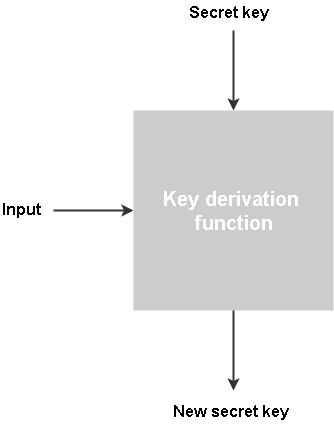
\includegraphics[width=8cm]{figures/kdf.png}
 	\caption{Key derivation function}
 	\label{fig:kdf}
 \end{figure}


A core concept in the Double Ratchet algorithm is KDF chains which build a chain of secret keys using KDF \cite{doubleratchet}. 


\subsubsection{Signal Protocol}

The Signal Protocol provides end-to-end encryption and was developed in 2013 and was first introduced in the app TextSecure\footnote{https://en.wikipedia.org/wiki/TextSecure}.

The Signal Protocol consists of two parts; The \emph{Triple Diffie-Hellman protocol} (TripleDH) and the Double Ratchet algorithm.

\paragraph{Triple Diffie-Hellman protocol}\label{tripledh}
Before the Double Ratchet algorithm can be used the two parties communicating need to agree on a shared secret key. In the Signal protocol this is achieved with Triple Diffie-Hellman protocol \emph{(TripleDH)}.

The Triple Diffie-Hellman protocol is a \emph{key agreement protocol}. It involves a server and two parties; Alice and Bob. 

The TripleDH protocol is characterized by three phases:

\begin{enumerate}
	\item \emph{Publishing keys:} A identity key and several prekeys belonging to Bob is published by him to a server.
	\item \emph{Sending initial message:} Alice sends an initial message to Bob. A prekey bundle is obtained by Alice from the server in order to send an initial message to Bob.
	\item \emph{Receiving initial message:} Alice's message is received and processed by Bob.
\end{enumerate}

\subparagraph{Publishing keys}
Bob needs to register a \emph{prekey bundle} to the server if he wants Alice to be able to send him messages. Alice will likewise have registered a prekey bundle so anyone can to anyone wants to start a message conversation with her.  
The prekey bundle exists of:

\begin{itemize}
	\item Identity key \emph{IK\textsubscript{B}}. This key is only published once by Bob.
	\item Signed prekey \emph{SPK\textsubscript{B}}. This key is reuploaded again after some period of time (eg. after each week or each month). 
	\item Prekey signature \emph{Sig(IK\textsubscript{B}, Encode(SPK\textsubscript{B}))}. This key is also reuploaded again like the signed prekey.
	\item Set of one-time prekeys \emph{(OPK\textsubscript{B}\textsuperscript{1}, OPK\textsubscript{B}\textsuperscript{2}, OPK\textsubscript{B}\textsuperscript{3}, ...)}. These keys are uploaded by Bob occasionally. Bob is informed by the server when there are few one-time prekeys left. 
	
	To ensure forward secrecy the private key of the one-time prekeys are deleted once Bob received messages that uses them. The signed prekey is deleted as well. However Bob might hold on to it for some time to get the messages that was delayed.  
\end{itemize}

\subparagraph{Sending initial message}
Alice retrieves Bobs public keys from the server. She receives one of Bob's single one-time prekey. The server deletes the one-time prekey that was send. It might be the case that all the one-time prekeys at the server has been used \cite{tripledh}.  


Alice verifies the prekey signature if the verification fails the protocol is aborted or else the following public keys are provided to generate a shared secret:

\begin{itemize}
	\item Identity key \emph{IK\textsubscript{A}}. Her own identity key. 
	\item Ephemeral key \emph{EK\textsubscript{A}}. The public key from a generated ephemeral key pair.
\end{itemize}


To generate the shared secret the following calculations are made:

\[DH_1 = DH(IK_A, SPK_B)\]
\[DH_2 = DH(EK_A, IK_B) \]
\[DH_3 = DH(EK_A, SPK_B)\]
\[DH_4 = DH(EK_A, OPK_B)\]
\[SK = KDF(DH_1 || DH_2 || DH_3 || DH_4)\]

There are performed atleast three Diffie-Hellman where \emph{DH\textsubscript{4}} is optional depending on if the server had more one-time prekeys.

Authentication is provided by \emph{DH\textsubscript{1}} and \emph{DH\textsubscript{2}} while \emph{DH\textsubscript{3}} and \emph{DH\textsubscript{4}} provides forward secrecy.

The figure \ref{tripledh} illustrates the calculations. 


\begin{figure}[H]
	\centering
	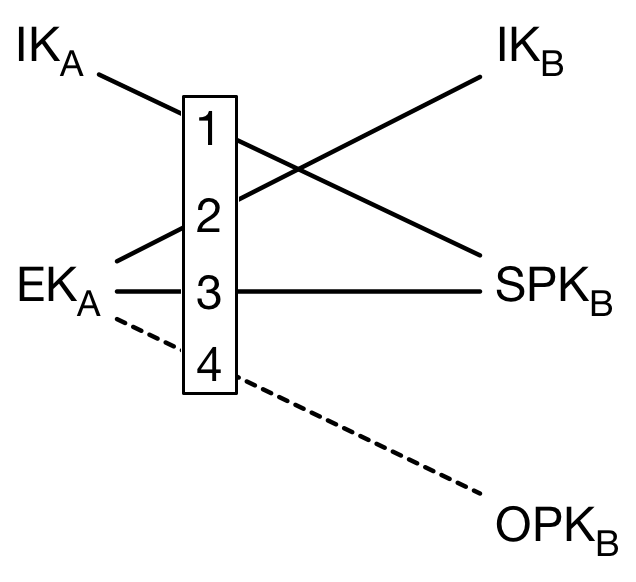
\includegraphics{figures/tripledh.png}
	\caption{Calculations of DH1-DH4 \cite{tripledh}.}
	\label{fig:tripledh}
\end{figure}

Alice then deletes the DH values and her private key associated to the ephemeral key to uphold forward secrecy and sends the initial message to Bob which consists of \cite{tripledh}: 

\begin{itemize}
	\item Cypher text with AEAD encryption  \footnote{https://en.wikipedia.org/wiki/Authenticated\_encryption} with \emph{associated data} using her own and Bob's identity keys.
	\item Her identity key \emph{IK\textsubscript{A}}.
	\item Her ephemeral key \emph{EK\textsubscript{A}}.
	\item Some identifiers to which of Bob's prekeys she used.
	
\end{itemize} 


\subparagraph{Receiving initial message}

When Bob receives Alice's initial message he performs the exact same calculations in phase two and derives the same shared secret key \emph{SK}.

Bob then decrypts the cypher text with the shared key and \emph{associated data} using his own and Alice's identity keys. If the decryption fails the protocol is aborted and \emph{SK} is deleted. Otherwise the protocol is complete and Bob deletes the one-time private prekey. 
The shared secret key can then be used for the Double Ratchet algorithm \cite{tripledh}.  

\paragraph{Double Ratchet algorithm}

After a shared secret key has been established the Double Ratchet algorithm can then be used to send and receive encrypted messages.

Each party has three chains; root chain, sender chain and receive chain. The chains are KDF chains and will take two keys as input (a KDF chain key and some other input key) and output new two keys (a new KDF chain key and some other output key). The KDF chain is illustrated in figure \ref{symkeyratchet}.

The algorithm has a \emph{Diffie-Hellman ratchet} step and \emph{symmetric ratchet} step and the chains are used across both steps.

\begin{itemize}
	\item \emph{Diffie-Hellman ratchet:} The parties exchanges new Diffie-Hellman public keys with the messages being sent. New secrets are then derived using Diffie-Hellman (DH). The secret that DH outputs is used as input to the root chain. The root chain then output new chain keys for the receiving and sending chains. 
	
	\item \emph{Symmetric ratchet:} The sending and receiving chains uses the chain keys derived from the root chain and for each message sent and received the chains are advanced. The output from the receiving and sending chains are keys for encrypting or decrypting messages. 
\end{itemize}


\subparagraph{Symmetric ratchet}
The symmetric ratchet provides message key through the receiving and sending chains. A message key is used for encryption or decryption of a message.

In the symmetric ratchet a single ratchet step is the calculation of the next key chain and message key. The inputs are the current chain key and a constant. Figure \ref{fig:symkeyratchet} illustrates two steps in a symmetric ratchet.

\emph{Forward secrecy} is provided since KDF is a one-way function and it is not possible to go backward and get the input chain key from the output chain key. However since the other input is simply a constant all future keys chain keys and message keys can be derived from an older chain key more specifically there is lack of backward secrecy.


\begin{figure}[H]
	\centering
	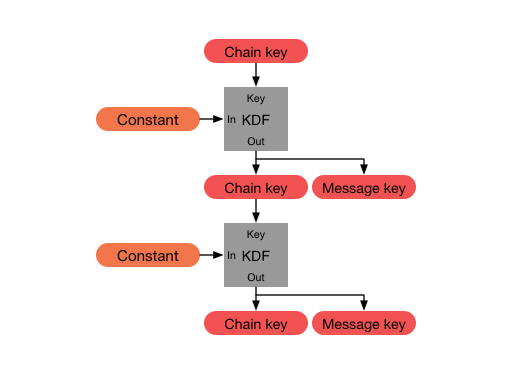
\includegraphics[width=10cm]{figures/symmetrickeyratchet.png}
	\caption{Symmetric key ratchet \cite{doubleratchet}.}
	\label{fig:symkeyratchet}
\end{figure}


\newpage
\subparagraph{Diffie-Hellman ratchet}

Double ratchet provides backward secrecy by comining the Symmetric ratchet with a Diffie-Hellman ratchet hence the name \emph{Double Ratchet}.

Every message from either party begins with a header which contains the sender's current ratchet public key. Whenever a new ratchet public key is received a new ratchet key pair is generated; a secret is derived through Diffie-Hellman with the input being the received ratchet public key and the ratchet private key from the new generated key pair.

Alice starts a conversation with Bob and uses his published public key as a ratchet public key. Alice then generates a new ratchet key pair and derives a shared secret key using Diffie-Hellman and would that as input to her \emph{sending chain}. Alice then sends her new ratchet public key to Bob. At the receiving end Bob derives the same shared secret which would be the input to his \emph{receiving chain}. Alice's sending chain and Bob's receiving chain share the same secret hence he can derive the message key and decrypt the message sent from Alice. When Bob sends a reply to Alice he would generate a new ratchet key pair and derive a new secret which would be input to his \emph{sending chain}.

Figure \ref{fig:dhratchet1} shows an ongoing message exchange with new secrets being derived and the sending and receiving chains being advanced.

\begin{figure}[H]
	\centering
	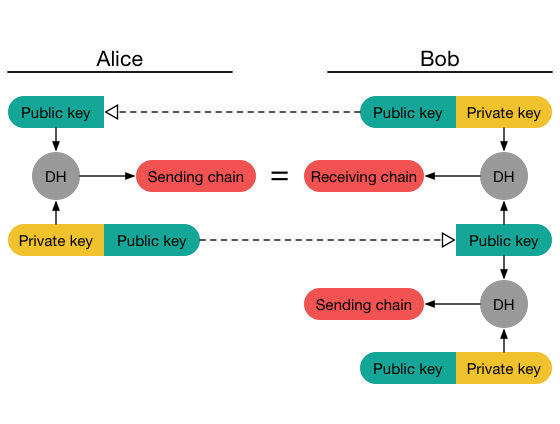
\includegraphics[width=9cm]{figures/dhratchet5.png}
	\caption{Diffie-Hellman ratchet \cite{doubleratchet}.}
	\label{fig:dhratchet1}
\end{figure}


When Alice receive the reply from Bob she would perform the exact same steps. This ultimately results in a continous loop of generating new ratchet key pairs and using Diffie-Hellman to derive the same shared secret key. A continuation is shown in figure \ref{fig:dhratchet2}

\begin{figure}[H]
	\centering
	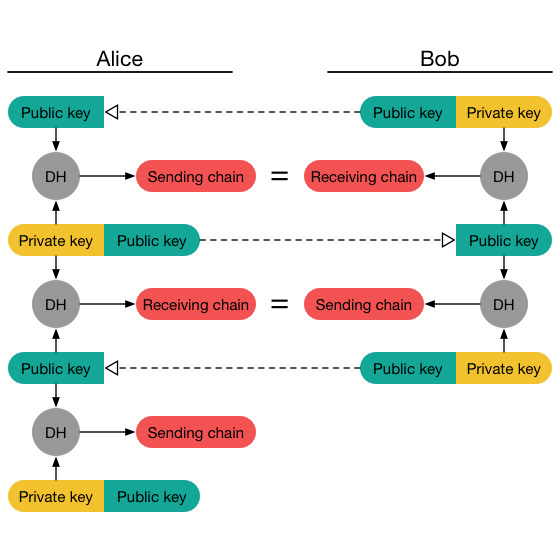
\includegraphics[width=9cm]{figures/dhratchet6.png}
	\caption{Continuation of Diffie-Hellman ratchet  \cite{doubleratchet}.}
	\label{fig:dhratchet2}
\end{figure}


As mentioned in the beginning of the Double Ratchet section the Diffie-Hellman ratchet does have a root chain which would provide inputs to the sending and receiving chains. A more correct view of the process in Diffie-Hellman is shown in figure \ref{fig:dhratchetcon}. 


\begin{figure}[H]
	\centering
	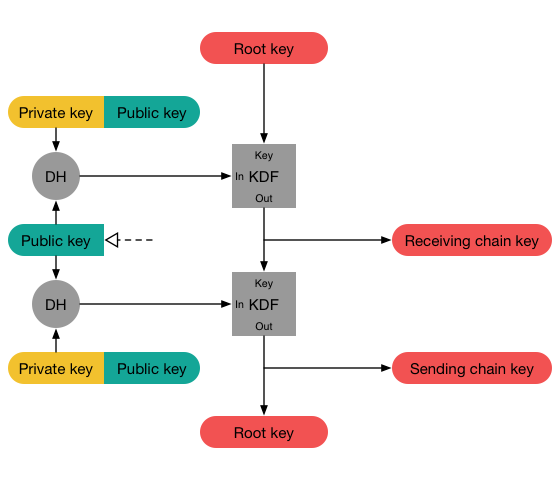
\includegraphics[width=9cm]{figures/dhratchet7.png}
	\caption{Diffie-Hellman ratchet 7 \cite{doubleratchet}.}
	\label{fig:dhratchetcon}
\end{figure}

\paragraph{Double ratchet}

When combining Diffie-Hellman ratchet and symmetric-key ratchet the result is the Double ratchet.

\begin{itemize}
	\item When sending or receiving a message the corresponding message key is derived by performing a symmetric-key ratchet step.
	\item Upon receiving a new ratchet public key the Diffie-Hellman ratchet step performed right before the symmetric-key ratchet step with the goal of replacing old chain keys with new ones.  
\end{itemize}

Assume that the message exchanged is a continuation from the TripleDH key exchange described in section \ref{tripledh}. Alice had sent an initial message. The initial ratchet public key would be Bob's signed prekey \emph{SPK\textsubscript{B}} and the new ratchet key pair would be the Alice's ephemeral key pair that she generated. Alice calculated a shared secret which is the \emph{root key}. She then generates a new ratchet key pair and takes the output from Diffie-Hellman and use it as input for the \emph{root chain}. The root chain then outputs a new root key \emph{RK} and a sending chain key {CK}.

The figure \ref{doubleratchet1} depicts this with a view of Alice's chains.


\begin{figure}[H]
	\centering
	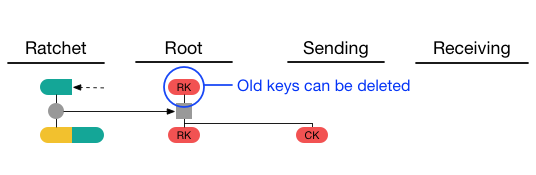
\includegraphics[width=10cm]{figures/doubleratchet1.png}
	\caption{Double ratchet 1 \cite{doubleratchet}.}
	\label{fig:doubleratchet1}
\end{figure}

When Alice then sends a message \emph{A1} the symmetric-key ratchet step will return a new chain key and a message key. The message can then be encrypted with the message key.

\begin{figure}[H]
	\centering
	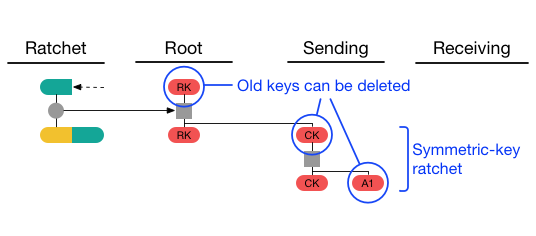
\includegraphics[width=10cm]{figures/doubleratchet2.png}
	\caption{Double ratchet 2 \cite{doubleratchet}.}
	\label{fig:doubleratchet2}
\end{figure}

Next Alice receives a message \emph{B1} from Bob. The message header contains a new ratchet public key and a Diffie-Hellman ratchet step is performed. New sending and receiving chain keys are derived and followed by a symmetric-key ratchet step to derive the receiving message key to decrypt the message.

\begin{figure}[H]
	\centering
	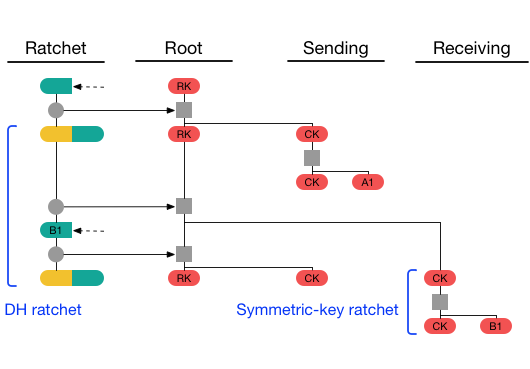
\includegraphics[width=10cm]{figures/doubleratchet3.png}
	\caption{Double ratchet 3 \cite{doubleratchet}.}
	\label{fig:doubleratchet3}
\end{figure}


\newpage
\section{Matrix}
Matrix is a set of open APIs for open-federated Instant Messaging (IM), Voice over IP (VoIP) and Internet of Things (IoT) communication, designed to create and support a new global real-time communication ecosystem. The intention is to provide an open decentralised pubsub layer for the internet for securely persisting and publishing/subscribing JSON objects. 
% https://www.youtube.com/watch?v=-ofZMnKkp_Y 5:00 , 18:30

\subsection{How does it work?}
Here are three Matrix homeservers, each with one client connected. The clients are all participating in the same Matrix room, which is synchronised across the three participating servers. 

Alice sends a JSON message to a room on her homeserver. 

Alice's homeserver adds the JSON to its graph of history, linking it to the most recent unlinked object(s) in the graph.The server then signs the JSON including the signatures of the parent objects to calculate a tamper-resistent signature for the history.

The server then sends the signed JSON over HTTPS to any other servers which are participating in the room.

The destination servers perform a series of checks on the message:
\begin{itemize}
	\item Validate the message signature to protect against tampering with history
	\item Validate the HTTP request's auth signature to protect against identity spoofing
	\item Validate whether Alice's historical permissions allow her to send this particular message
\end{itemize}

If these checks pass, the JSON is added to the destination servers' graphs.

Destination clients receive Alice's message with a long-lived GET request. (Clients are free to implement more efficient transports than polling as desired).

\begin{figure}[H]
	\centering
	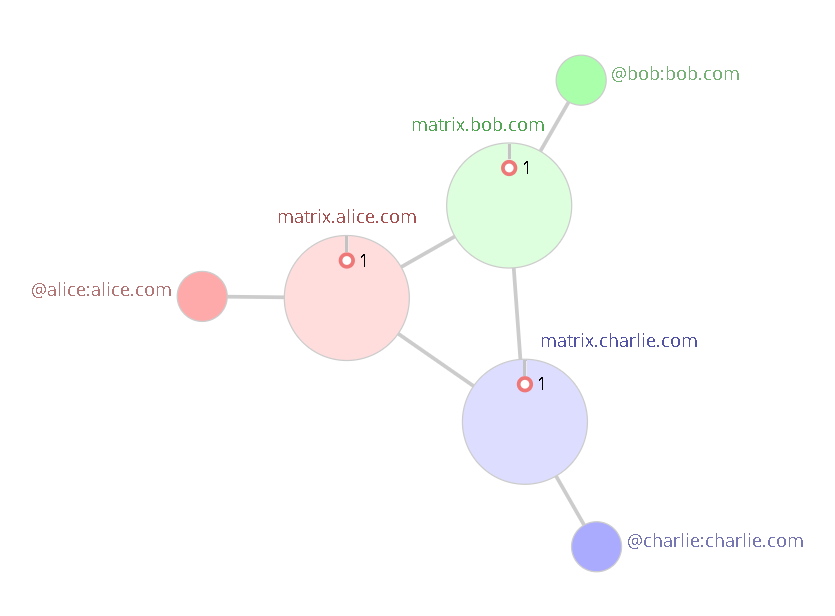
\includegraphics[width=9cm]{figures/matrix1.png}
	\caption{ Matrix \cite{matrixhome}.}
	\label{fig:matrix1}
\end{figure}

Bob sends a response to Alice's message, and his server adds his message into his copy of the room's history, linking it to the most recent unlinked object in the graph - Alice's last message.

Meanwhile, Charlie also responds to Alice's message - racing with Bob's message. Alice, Bob and Charlie's homeservers all have different views of the message history at this point - but Matrix is designed to handle this inconsistency.

\begin{figure}[H]
	\centering
	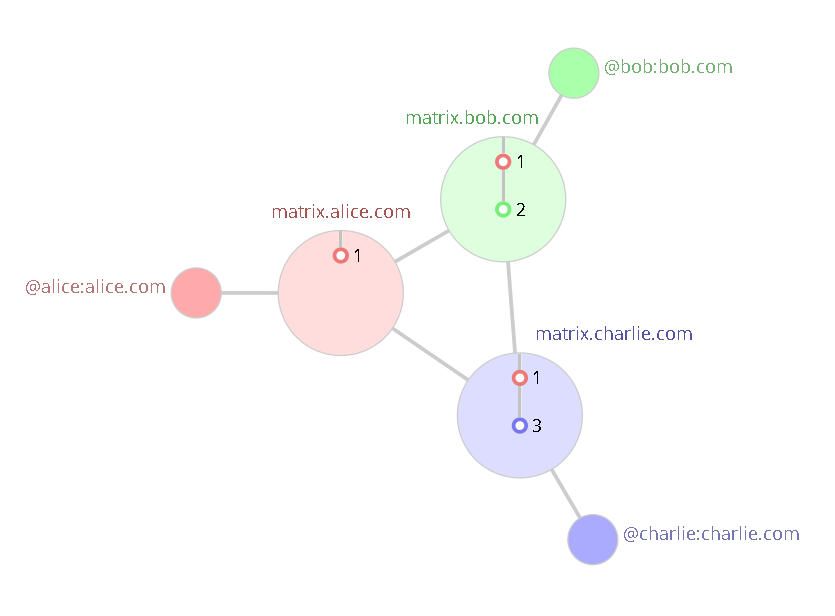
\includegraphics[width=9cm]{figures/matrix2.png}
	\caption{ Matrix \cite{matrixhome}.}
	\label{fig:matrix2}
\end{figure}

Bob's homeserver relays his message through to Alice and Charlie's servers, who accept it. At this point Alice and Bob are in sync, but Charlie's room history has split - both messages 2 and 3 follow on from message 1. This is not a problem; Charlie's client will be told about Bob's message and can handle it however it chooses.


\begin{figure}[H]
	\centering
	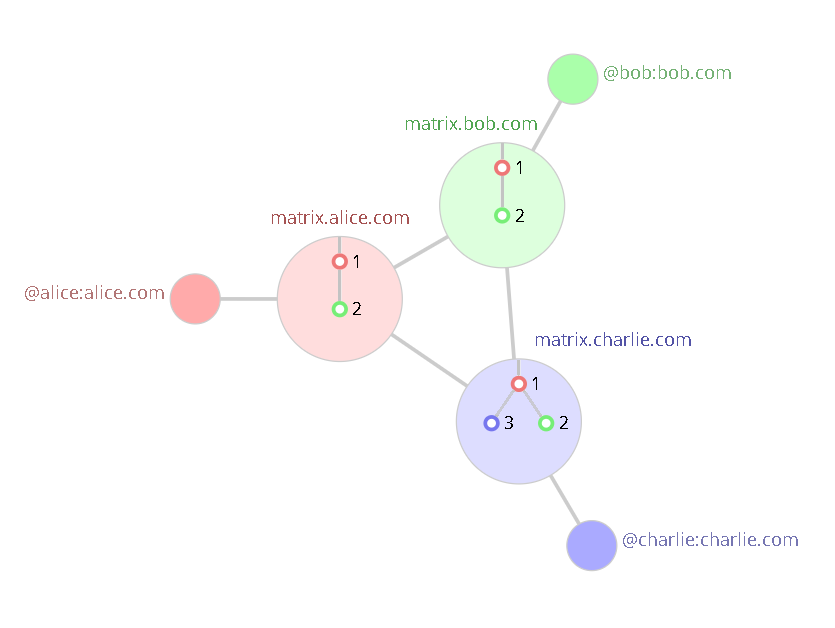
\includegraphics[width=9cm]{figures/matrix3.png}
	\caption{ Matrix \cite{matrixhome}.}
	\label{fig:matrix3}
\end{figure}

 
Charlie's homeserver relays his message through as well, at which point all 3 servers have a consistent view of history again (including the race between Bob and Charlie). All three clients have seen all three messages, and the room history is now back in sync across the participating servers.


\begin{figure}[H]
	\centering
	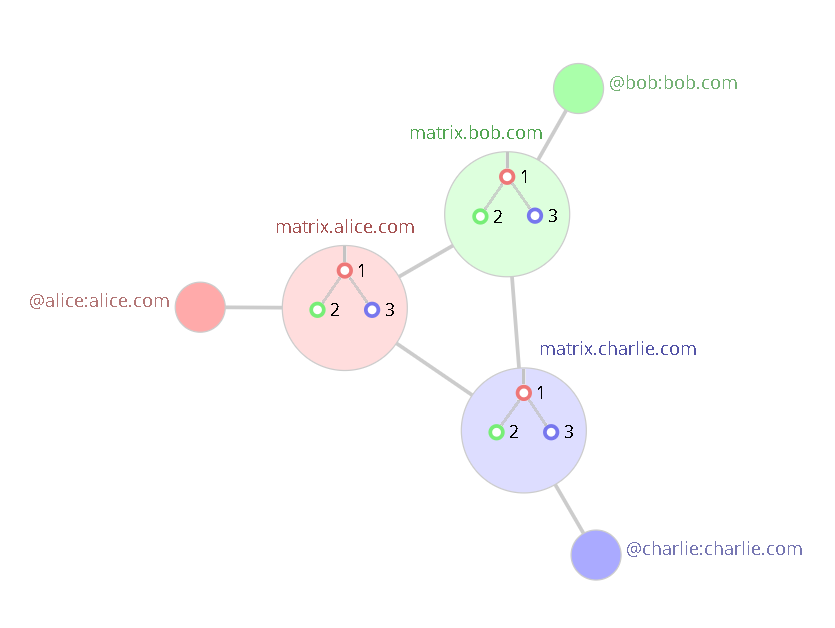
\includegraphics[width=9cm]{figures/matrix4.png}
	\caption{ Matrix \cite{matrixhome}.}
	\label{fig:matrix4}
\end{figure}

Later on, Alice sends another message - her homeserver adds it to her history, and links it to the most recent unlinked objects in the graph: Bob and Charlie's messages. This effectively merges the split in history and asserts the integrity of the room (or at least her view of it). 

Alice's message is then relayed to the other participating servers, which accept it and update their own history with the same rules, ensuring eventual consistency and integrity of the distributed room.

\begin{figure}[H]
	\centering
	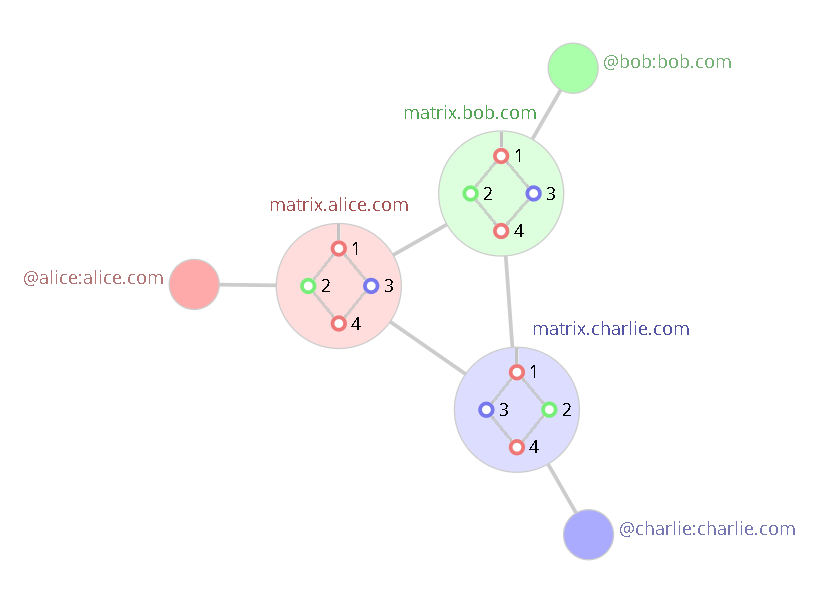
\includegraphics[width=9cm]{figures/matrix5.png}
	\caption{ Matrix \cite{matrixhome}.}
	\label{fig:matrix5}
\end{figure}

\subsection{Architecture}
Matrix defines APIs for synchronising extensible JSON objects known as "events" between compatible clients, servers and services. Clients are typically messaging/VoIP applications or IoT devices/hubs and communicate by synchronising communication history with their "homeserver" using the "Client-Server API". Each homeserver stores the communication history and account information for all of its clients, and shares data with the wider Matrix ecosystem by synchronising communication history with other homeservers and their clients.

Clients typically communicate with each other by emitting events in the context of a virtual "room". Room data is replicated across all of the homeservers whose users are participating in a given room. As such, no single homeserver has control or ownership over a given room. Homeservers model communication history as a partially ordered graph of events known as the room's "event graph", which is synchronised with eventual consistency between the participating servers using the "Server-Server API". This process of synchronising shared conversation history between homeservers run by different parties is called "Federation". Matrix optimises for the Availability and Partitioned properties of CAP theorem at the expense of Consistency.

\begin{figure}[H]
	\centering
	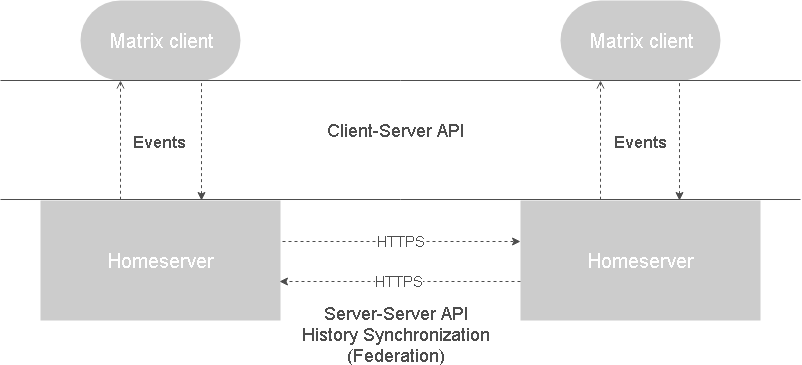
\includegraphics[width=12cm]{figures/matrix_architecture.png}
	\caption{ Matrix conceptual architecture \cite{matrixspec}.}
	\label{fig:matrix_architecture}
\end{figure}

\subsubsection{Event}

All data exchanged over Matrix is expressed as an "event". Typically each client action (e.g. sending a message) correlates with exactly one event. Each event has a type which is used to differentiate different kinds of data. type values MUST be uniquely globally namespaced following Java's package naming conventions, e.g. com.example.myapp.event. The special top-level namespace m. is reserved for events defined in the Matrix specification - for instance m.room.message is the event type for instant messages. Events are usually sent in the context of a "Room".

Events exchanged in the context of a room are stored in a directed acyclic graph (DAG) called an "event graph". The partial ordering of this graph gives the chronological ordering of events within the room. Each event in the graph has a list of zero or more "parent" events, which refer to any preceding events which have no chronological successor from the perspective of the homeserver which created the event.

Typically an event has a single parent: the most recent message in the room at the point it was sent. However, homeservers may legitimately race with each other when sending messages, resulting in a single event having multiple successors. The next event added to the graph thus will have multiple parents. Every event graph has a single root event with no parent.

\subsubsection{Room}
A room is a conceptual place where users can send and receive events. Events are sent to a room, and all participants in that room with sufficient access will receive the event. Rooms are uniquely identified internally via "Room IDs", which have the form:

\[!r00m1d:matrix.org\]

There is exactly one room ID for each room. Whilst the room ID does contain a domain, it is simply for globally namespacing room IDs. The room does NOT reside on the domain specified.


\begin{figure}[H]
	\centering
	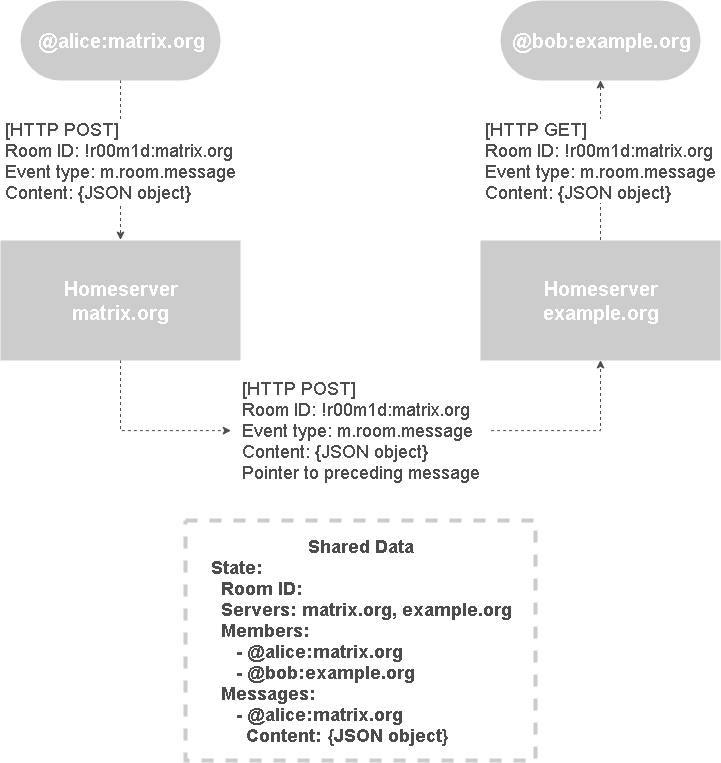
\includegraphics[width=11cm]{figures/matrix_room.png}
	\caption{ Matrix conceptual architecture \cite{matrixspec}.}
	\label{fig:matrix_room}
\end{figure}

Federation maintains shared data structures per-room between multiple homeservers. The data is split into message events and state events.

\subparagraph{Message events}
These describe transient 'once-off' activity in a room such as an instant messages, VoIP call setups, file transfers, etc. They generally describe communication activity.

\subparagraph{State events}
These describe updates to a given piece of persistent information ("state") related to a room, such as the room's name, topic, membership, participating servers, etc. State is modelled as a lookup table of key/value pairs per room, with each key being a tuple of state\_key and event type. Each state event updates the value of a given key.
The state of the room at a given point is calculated by considering all events preceding and including a given event in the graph. Where events describe the same state, a merge conflict algorithm is applied. The state resolution algorithm is transitive and does not depend on server state, as it must consistently select the same event irrespective of the server or the order the events were received in. Events are signed by the originating server (the signature includes the parent relations, type, depth and payload hash) and are pushed over federation to the participating servers in a room, currently using full mesh topology. Servers may also request backfill of events over federation from the other servers participating in a room.

\subsection{Matrix specification}

Matrix defines a set of open APIs for decentralised communication, suitable for securely publishing, persisting and subscribing to data over a global open federation of servers with no single point of control. Uses include Instant Messaging (IM), Voice over IP (VoIP) signalling, Internet of Things (IoT) communication, and bridging together existing communication silos - providing the basis of a new open real-time communication ecosystem. 

Matrix two main API specification; Client/Server API and Federated API. Any Matrix SDK implements the API defined at the Client/Server API specification. If a custom homeserver was to be developed from scratch it would have to conform to the Federated API to be able to be a part of Matrix. 

\subparagraph{Client/Server API}
The client-server API provides a simple lightweight API to let clients send messages, control rooms and synchronise conversation history. It is designed to support both lightweight clients which store no state and lazy-load data from the server as required - as well as heavyweight clients which maintain a full local persistent copy of server state.

\subsection{End-to-end Encryption}
Privacy is particularly critical for a decentralized network like Matrix, where user data is replicated over all the servers participating in a room and so must be protected. Matrix provides state of the art end-to-end encryption in beta using the Olm and Megolm cryptographic ratchets, and ensuring that only explicitly authorized devices can participate in a conversation. 

Olm and Megolm are examined in section \ref{matrixeval}.


The end-to-end encryption is based on the Double Ratcet algorithm.


\begin{itemize}
	\item Provides 1:1 encrypted channels between pairs of devices via the Olm double ratchet 
	\item Supports group chats with hundreds of devices via the new Megolm shared ratchet, with either perfect forward secrecy or the ability to decrypt conversation history on new devices. 
	\item Supports multiple devices, tracking verification trust per-device to help spot interception.
\end{itemize}


Currently any apps built on matrix-js-sdk, matrix-ios-sdk or matrix-android-sdk support encryption, which is in beta as of March 2017.  The libolm library itself is considered stable however.




\newpage
\section{Information Flow Control} %mere konkret og teknisk
%Selvom jeg ikke kiggr på fx trafic analysis så er det vigtigt at nævne og påpege det ikkeer noget jeg løser

\subsection{The Lattice Model}
adsadsad

\subsection{Noninterference}
dasdsa

\subsection{Static policies}


sadsad
\subsection{Dynamic policies}
sadsadsad


\subsection{Declassification}
Taking some specific information and changing it to a lower security classification.

Identify: What to classify, who declassifies, where the declassification happens and when the declassification happens

\section{Summary}
